\section*{Exercice 185 -- Cinématique et RSG}
\setcounter{exo}{0}

Le solide \textbf{1} roule sans glisser sur le \textbf{0}. Le solide \textbf{2} est en glissière de direction $\vect{u}$ par rapport à \textbf{1}. On considère que le mouvent est plan. 
On note $\theta=\angl{x}{u}$, $\vect{AP}=\lambda(t)\vect{u}$ et $\vect{HA}=R\vect{y}$.

\begin{center}
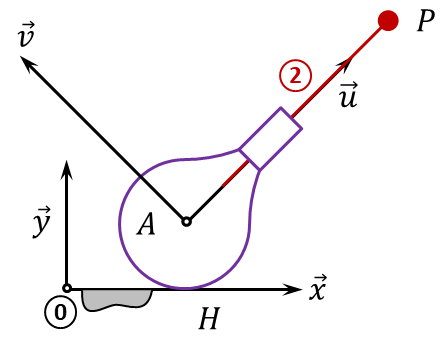
\includegraphics[width=.7\linewidth]{033_01}
\end{center}

\subparagraph{}
\textit{Déterminer $\vectv{P}{2}{0}$.}
\ifprof
\begin{corrige}

\end{corrige}
\else
\fi

\subparagraph{}
\textit{Déterminer $\vectg{P}{2}{0}$.}
\ifprof
\begin{corrige}

\end{corrige}
\else
\fi
